\section{Beam Polarizations}

Time-dependent relative beam polarizations are obtained from the pC CNI
polarimeter and normalized by the H-jet polarimeter. pC measurements are made
every few hours during a fill, while the H-jet polarimeter is taking data
almost continuously.

During the 2005 RHIC run pC measurements were generally performed with
vertical targets at one location in \(x\), the horizontal coordinate in the
plane transverse to the beams. The intent was that the measurement be made at
the intensity peak. A small number of explicit polarization profile
measurements were also performed. A study of the normalized event rates
obtained by the polarimeter indicated that the target was occasionally
off-center relative to the beam. In the case of the blue beam, the
polarization showed no dependence on normalized event rate, nor any explicit
dependence on \(x\) in the profile measurements. In contrast, the yellow beam
polarization exhibited a significant normalized rate dependence as well as an
\(x\) dependence in the profile measurements. In the 2006 RHIC run scanning
profile measurements in \(x\) were executed for both beams as the normal mode
of operation as a result of this discovery.

The existence of a non-uniform polarization profile in the beam has
implications for the H-jet normalization procedure. The H-jet target is large
compared to the size of the beam and thus samples the average polarization,
while the pC target is small in one dimension. In order to relate the two one
needs to calculate an average beam polarization from the pC measurements,
which requires knowledge of the beam intensity and polarization profiles in
the transverse dimension orthogonal to the carbon strip. The data from the
2006 polarimeter measurements theoretically enables a direct extraction of
both profiles, but occasional problems with the target positioning render the
procedure somewhat unreliable.

The alternative approach employed by the CNI Polarimeter Group in both the
2005 and 2006 data analyses relies on the assumption that the beam intensity
and polarization profiles are Gaussian with independent widths, and that the
peak of the polarization profile is located at the center of the beam. Then
the polarization \(P\) and normalized event rate \(I\) are related by
%
\begin{equation}
  \frac{P}{P_{max}} = I^R, ~~~~ R=\left(\frac{\sigma_I}{\sigma_P}\right)^2.
  \label{eqn:polarization}
\end{equation}
%
\(P_{max}\) and \(R\) are free parameters determined in a fit to the data; the
average beam polarization in terms of these parameters is simply
%
\begin{equation}
  \langle P \rangle = \frac{P_{max}}{\sqrt{1+R}}
\end{equation}

After H-jet normalization, the polarization values reported to the experiments
must be weighted by the product of both beam intensities. Recall that the
value for \(P_{max}\) in \ref{eqn:polarization} already reflects the carbon
ribbon target's uniform cross section in one transverse dimension; the
polarization at the two-dimensional intensity peak is actually
\(P_{max}\sqrt{1+R}\), and the luminosity-weighted average beam polarization
assuming similarly-sized beams (\(\sigma_I^{blue} \approx \sigma_I^{yellow}\))
is then
%
\begin{equation}
  \langle P \rangle_{STAR} = \frac{P_{max} \sqrt{1+R}}{\sqrt{(1+R_x/2)(1+R_y/2)}}.
\end{equation}
%
In the typical pC running mode the carbon ribbon target is vertical, so the
\(R\) in the numerator is more precisely \(R_x\). The polarization profile is
usually much wider than the luminosity profile, so a binomial expansion leads
to
%
\begin{equation}
  \langle P \rangle_{STAR} = P_{max} \sqrt{\frac{1+R_x/2}{1+R_y/2}},
\end{equation}
and in the case where the polarization profiles are similar in both beams, the
luminosity-weighting correction term vanishes. Polarization profile
measurements in the vertical direction are statistically limited in both the
2005 and 2006 datasets but do not indicate any significant difference between
the horizontal and vertical polarization profiles. As a result, the analysis
sets the luminosity-weighting correction term to unity and includes a
systematic uncertainty term reflecting a possible difference in polarization
profiles in the two transverse dimensions.

The final results of fill-by-fill beam polarizations are shown in Figure
\ref{fig:beam-polarizations}. % something about uncertainties

% ok, so we get the average beam polarization by calculating Pmax and R from polarization v. event rate in the scans.  In 2006 that's easy, we have a scan each time.  In 2005, this is the global C_1X number for each beam extracted from the polarization v rate

% --- quality checks on carbon mode data
% width of carbon mass peak
% energy slope
% chi2 for bunch-by-bunch left-right asymmetries (poor chi2 == uncollimated beam)

% polarization values for experiments obtained by intensity^2 - weighted average of polarization profiles (right?  because polarization is different for different parts of the beam, and our events come from all parts of the beam, but mostly in the center).

\begin{figure}
  \subfloat[][2005 fills]{
    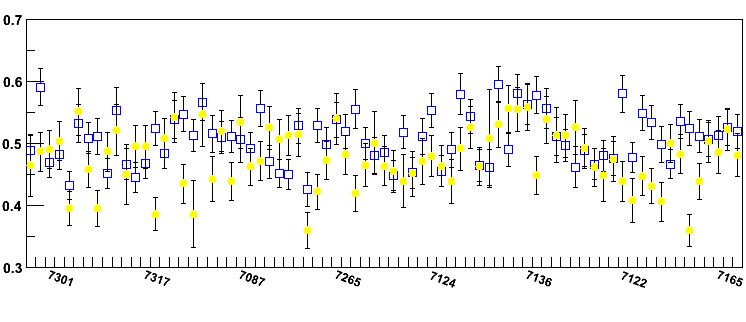
\includegraphics[width=1.0\textwidth]{figures/beam_polarizations_05}
  } \\
  \subfloat[][2006 fills]{
    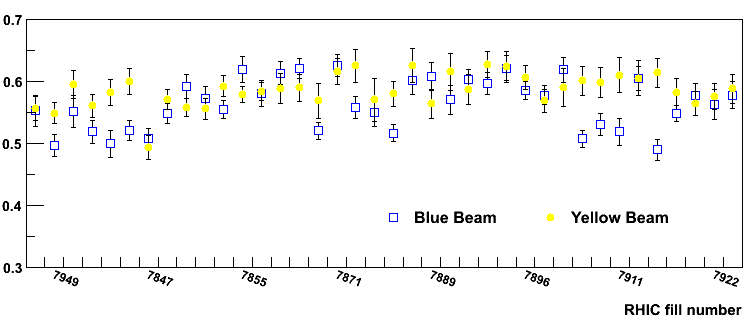
\includegraphics[width=1.0\textwidth]{figures/beam_polarizations_06}
  }
  \caption{RHIC beam polarizations for longitudinally polarized stores analyzed in this work.}
  \label{fig:beam-polarizations}
\end{figure}

\subsection{Polarization Vectors and Transverse Asymmetries}

